\begin{figure}\centering
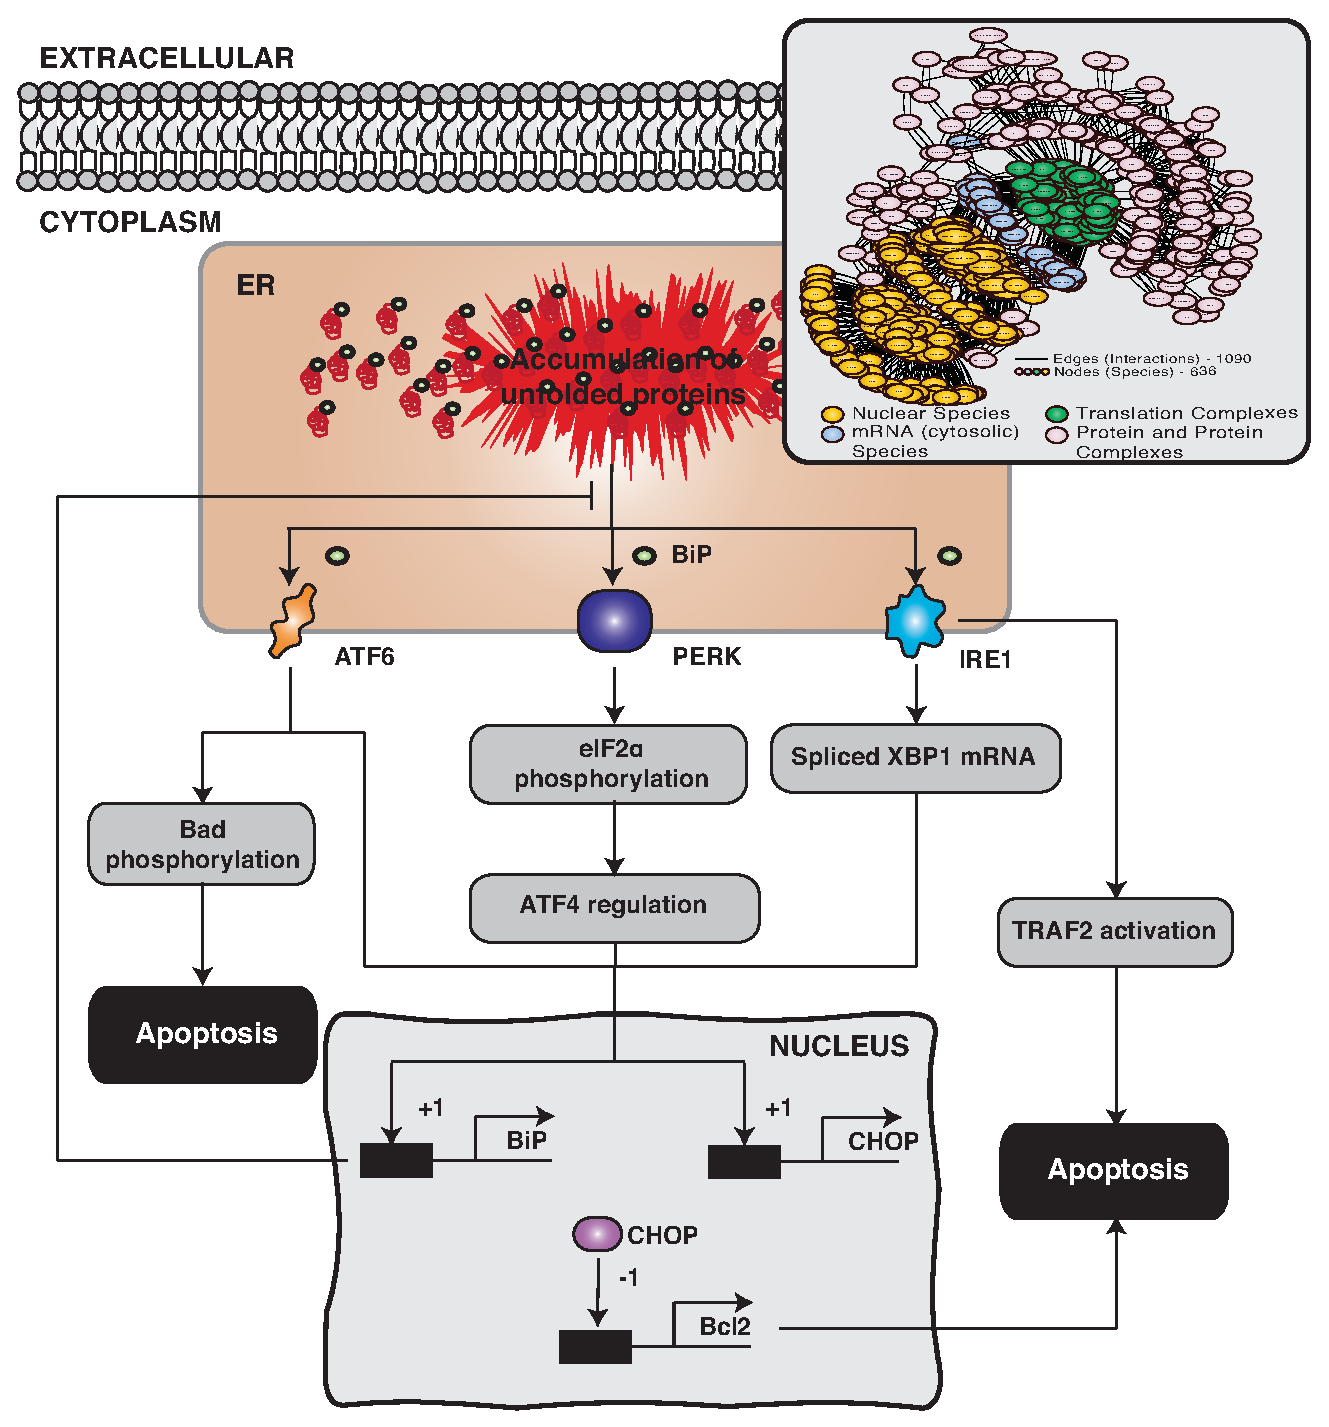
\epsfig{file=./Main_Figures/Pathway_F1.eps,width=0.8\textwidth}
	\caption{An array of cellular stressors can perturb the folding environment in the endoplasmic reticulum (ER) leading to unfolded or misfolded protein. In response to the folding imbalance, cells initiate the cytoprotective unfolded protein response (UPR). The problem of unfolded or misfolded proteins in the ER is addressed by increasing the folding capacity through the up-regulation of the expression of chaperone proteins, attenuating translation by regulating eIF2$\alpha$, and promoting the degradation of misfolded proteins through ER-associated degradation (ERAD). If UPR is unable to restore the folding balance, ER stress will eventually lead to apoptotic cell-death. The three signal transduction pathways mediating the unfolded protein response in higher eukaryotes. First, the PRKR-like ER kinase (PERK) pathway is initiated after BiP dissociation from PERK. While PERK transduces both pro- and anti-apoptotic signals, its main function is translation attenuation through the phosphorylation of eIF2$\alpha$. Next, the activating transcription factor 6 (ATF6) pathway is activated following BiP dissociation. ATF6 induces the expression of chaperones e.g., BiP as well as apoptosis effectors such as CHOP. Lastly, the inositol-requiring kinase 1 (IRE1) pathway is activated following BiP dissociation from IRE1. Activated IRE1 has both an endoribonuclease and a serine-threonine kinase activity that drive can pro-apoptotic signals. Inset: The UPR network consisted of 636 protein or mRNA species interconnected by 1090 interactions.}
	\label{fg:fig1}
\end{figure}

\begin{figure}\centering
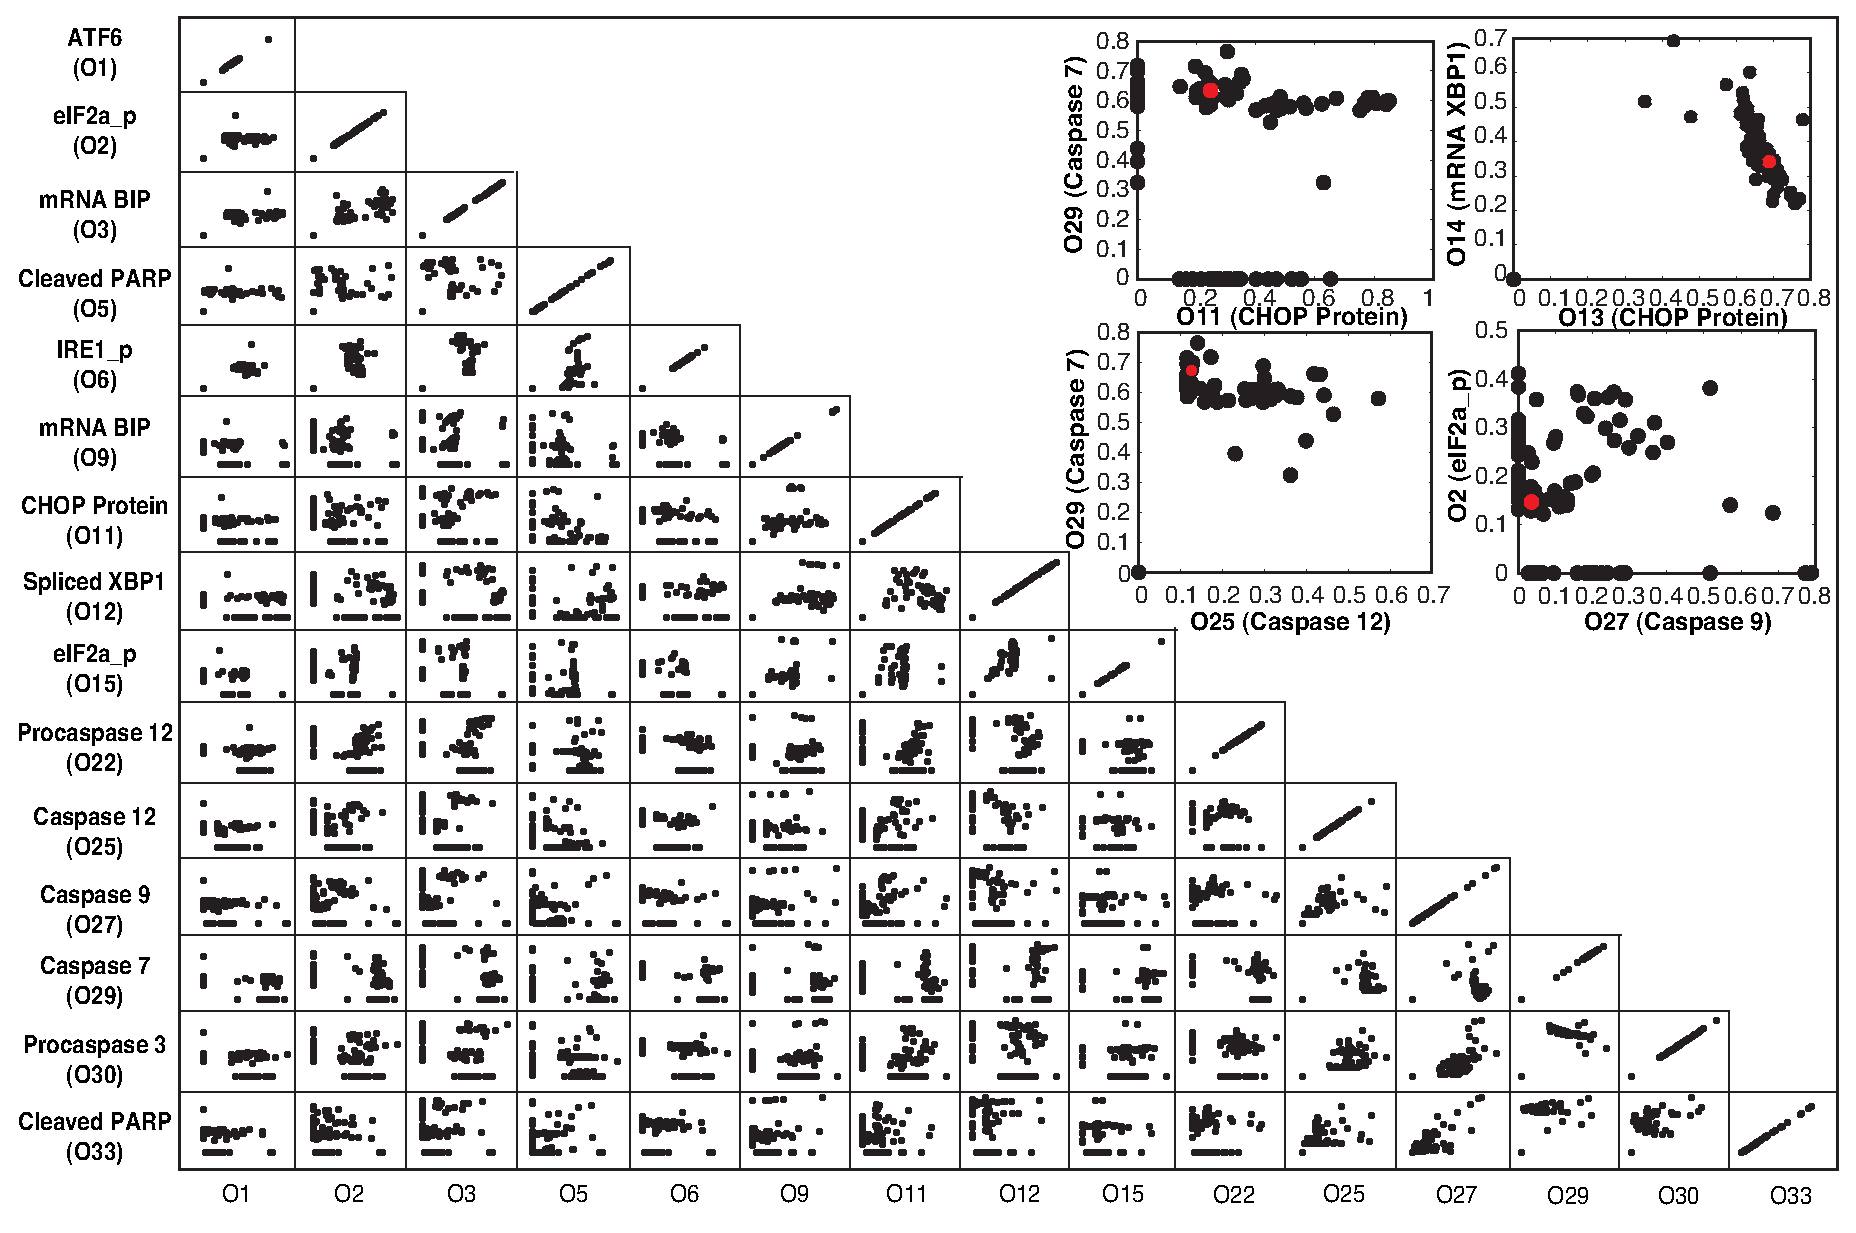
\epsfig{file=./Main_Figures/OBJ_F2.eps,width=1.0\textwidth}
	\caption{Objective function plot for selected training constrains (O1,O2,$\hdots$O33) for the UPR model population generated using POETs. Points denote separate models in the population. Several objectives exhibit clear Pareto fronts, e.g., O29 $\times$ O25. This suggests an inability to model both training constraints simultaneously or conflicts in the training data.}
	\label{fg:objective_plot}
\end{figure}

\begin{figure}\centering
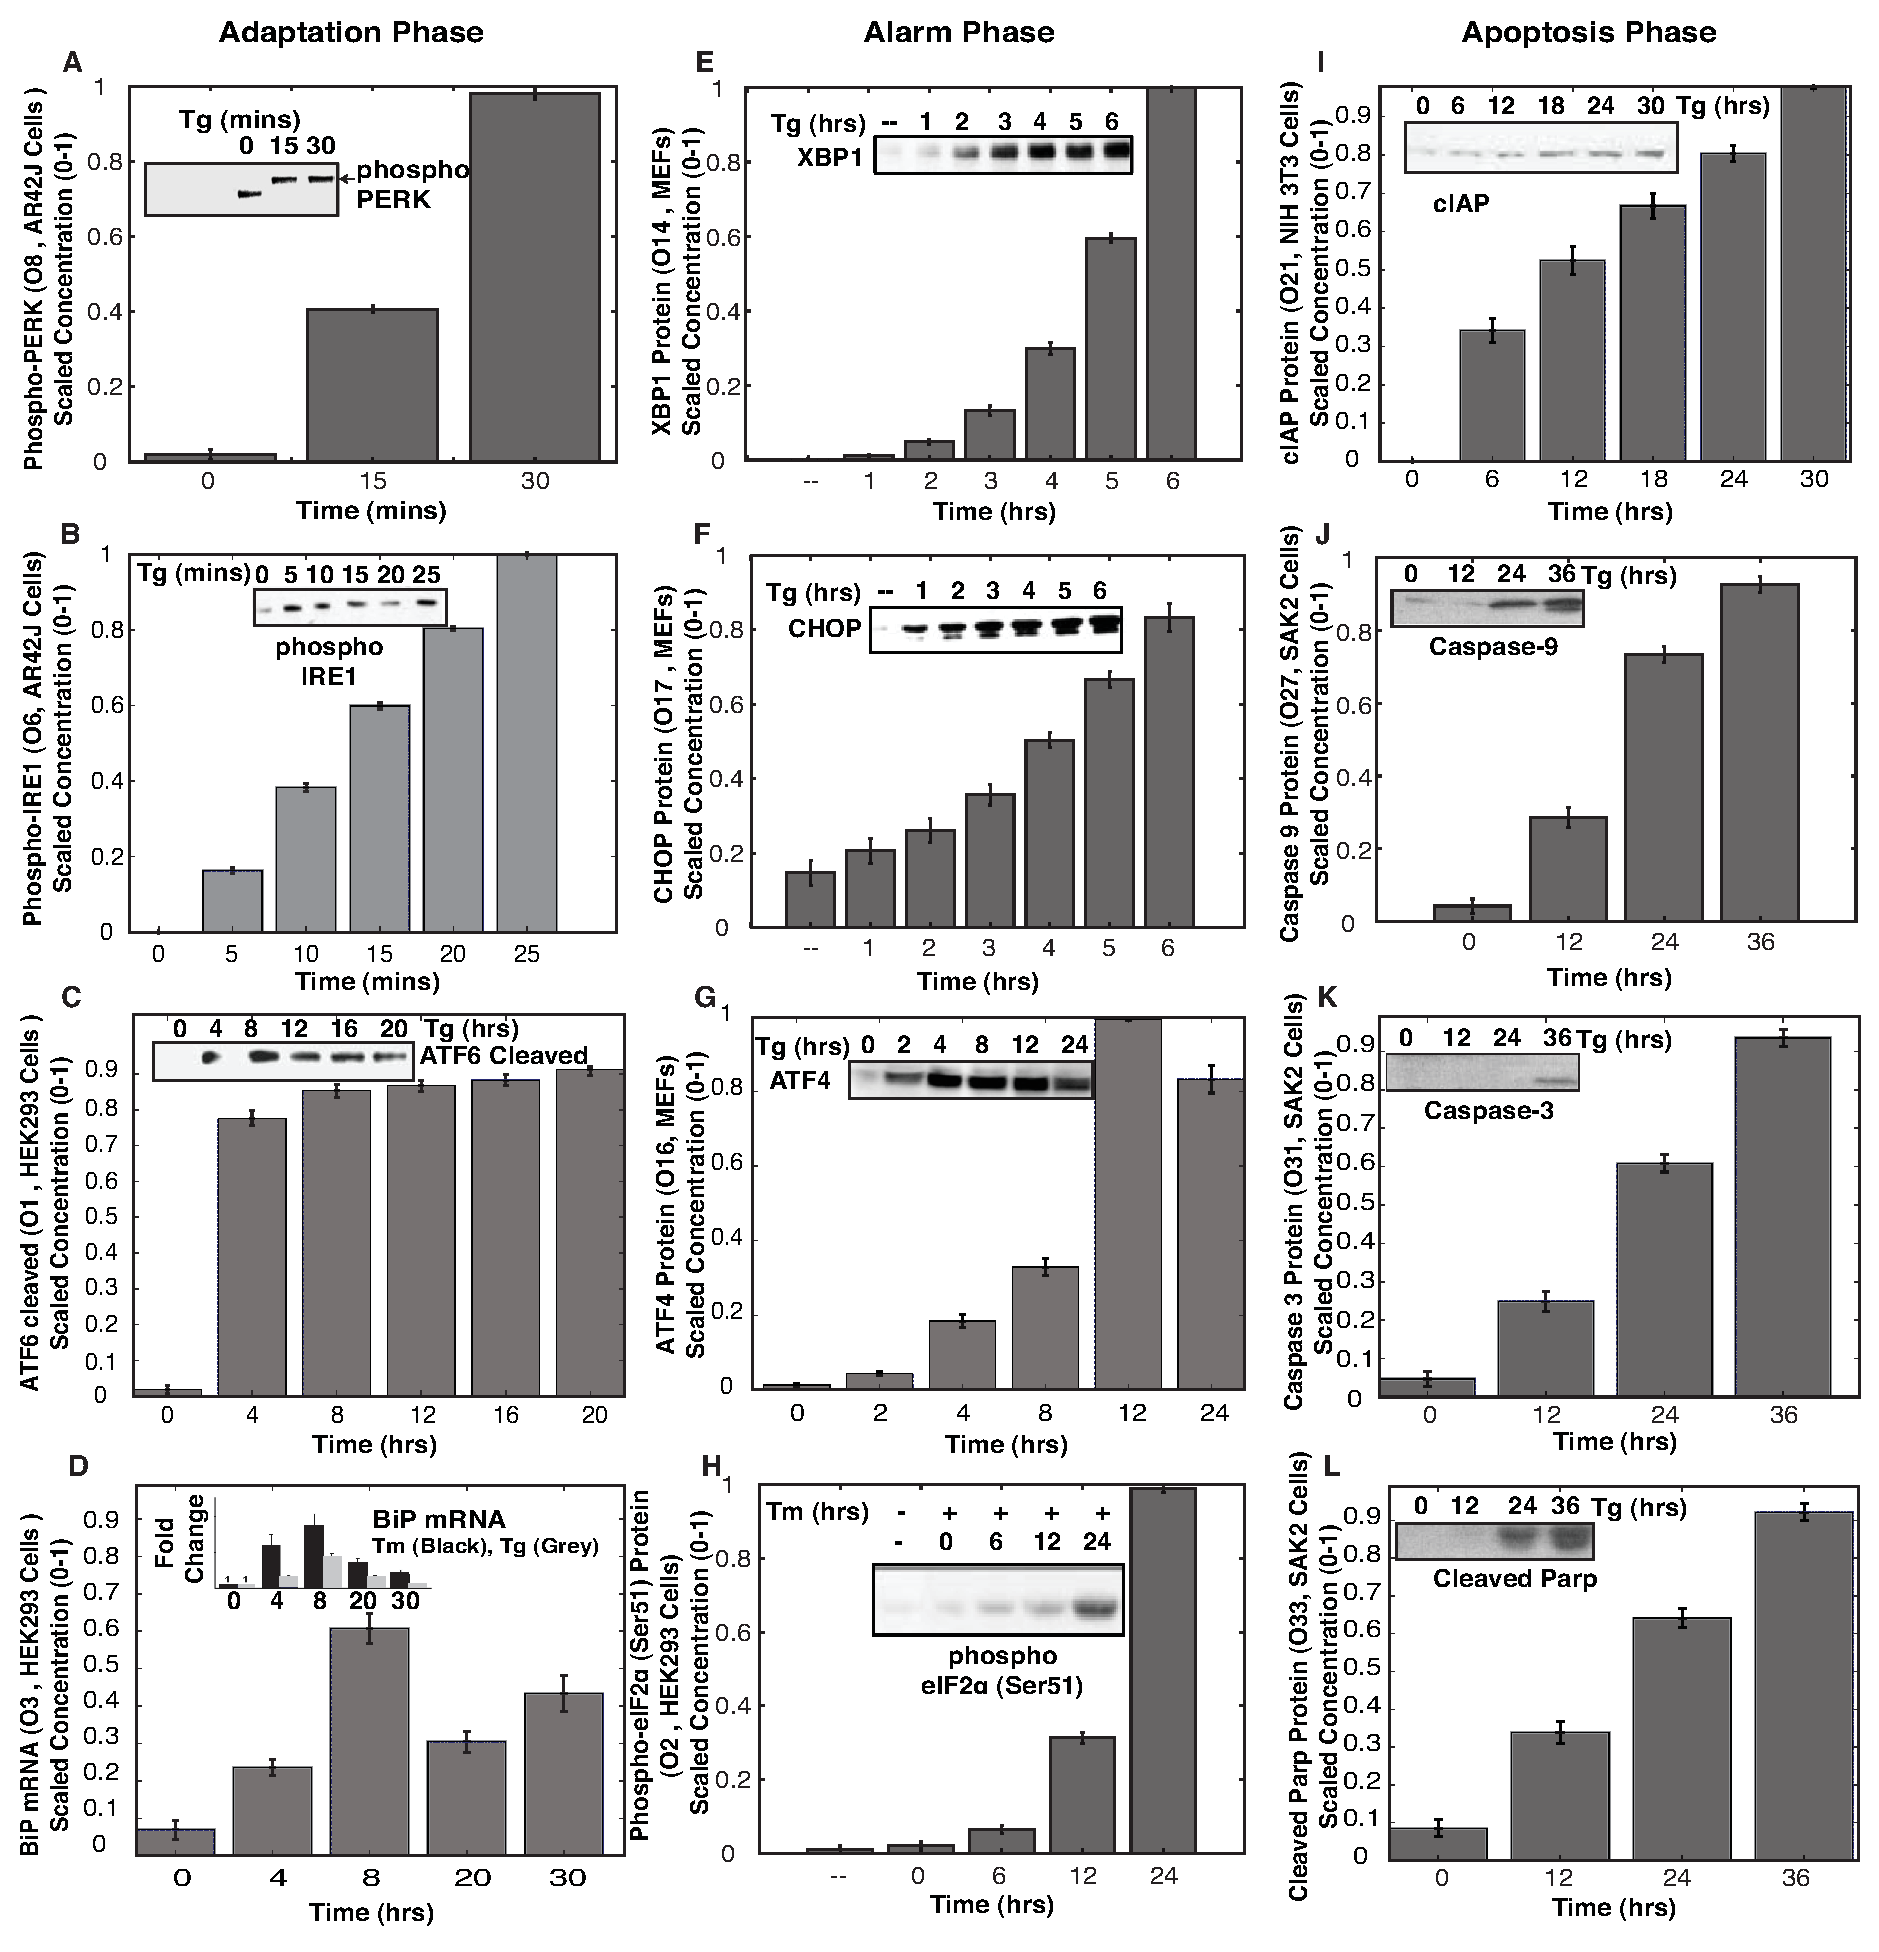
\epsfig{file=./Main_Figures/TRPR_F3.eps,width=1.0\textwidth}
	\caption{Simulations versus experimental data for selected objective functions following exposure to the ER-stress inducers Thapsigargin (Tg or Thaps) or Tunicamycin (TM). The first-column (A - D) denotes adaptation components, the second column (E - H) denotes alarm phase components, while the third column (I - L) denotes apoptosis phase components. Bars denote the scaled mean concentration computed over the ensemble, while the error bars describe one standard error.}
	\label{fg:simulation_comparison}
\end{figure}

\begin{figure}\centering
\epsfig{file=./Main_Figures/Proof_F4.eps,width=1.0\textwidth}
	\caption{Proof of concept simulation unfolded protein response activation. 
	\textbf{A:}UPR induction was controlled by manipulating the generation rate of unfolded or misfolded protein (qP) in the ER compartment. A step-change in qP from qP = 0.1 to qP = 100 was issued at approximately t = 0.1 hrs and then adjusted back to qP = 0.1 at t = 20 hrs.
	\textbf{B:}Flux through the PERK, ATF6 and IRE1 stress sensing branches as a function of time following a step change in misfolded protein generation.
	\textbf{C:}Simulated expression profile for the 59 genes in the model. The symbol UPROT denotes the level of unfolded protein.}
	\label{fg:proof_of_concept_simulation}
\end{figure}

\begin{figure}\centering
\epsfig{file=./Main_Figures/Flux_F5.eps,width=0.8\textwidth}
	\caption{Cross plot of the fluxes at P1-P5 as denoted in Figure 4: We tried to see is how the system behaves and how the system can recuperate from UPR dose when it is in the adaptation phase as compared to the apoptosis phase. (D) As compared to P1 (No-UPR Steady State), we see that early on at 1 hr after UPR dose there is a marked increase in ATF4 and CHOP regulation, ATF6 signaling along with unfolded protein sensing and degradation. These are hallmarks of the adaptation-alarm phase of the UPR response. (A) If we continue with the dose of UPR till around 25 hrs, we see the fluxes reach a steady state. This state is marked by increased BiP regulation, enhanced ATF4 transcriptional activity, increased mitochondrial membrane permeability and increased apoptotic fluxes. This state is similar to the Apoptotic phase of UPR, where in the cell has committed itself to apoptosis mediated cell death. (B) and (C) If we reduce the UPR load after the cell has committed to apoptosis (as in P3), we find that the cell continues to function similar to the UPR state even upon UPR load reduction after 25 hrs. There are certain aspects which are seen to reduce like IRE1-TRAF2 signaling, ASK1 activation. However not much difference is seen in terms of apoptotic fluxes, denoting the cell has committed itself to death and is in a point of no return. (E)-(F) On the contrary if we reduce the load of UPR in the adaptation-alarm phase (P4), we see that the cell can recuperate using its ERAD machinery and the regulation of BiP.}
	\label{fg:cross_plot_flux}
\end{figure}

\begin{figure}\centering
\includegraphics[width = 6.0in,height=5.5in]{./Main_Figures/Sens_F1.pdf}
	\caption{Rank-ordering of species sensitivities in the presence of UPR as a function of time.
	\textbf{Inset:} Rank-ordering of parameter sensitivity for UPR-induced versus normal conditions.
Points denote the mean ranking computed over N = 5 parameter sets from the model population, while error bars denote one standard deviation. Points are color-coded based based upon biological function.}
	\label{fg:fig5}
\end{figure}

\begin{figure}\centering
\epsfig{file=./Main_Figures/Rob_F7.eps,width=0.8\textwidth}
	\caption{Robustness analysis of the UPR network: A-B Phenotypic phase plane analysis for the the UPR model following structural perturbations. Coupling coefficients (area under the curve from the simulation with species removed dived by the wild-type simulation) for all 636 model species were calculated for the nominal parameter set following gene overexpression/knockout (A) and deletion of single network edges (B). Coupling coefficients of one indicate no change in a marker level following a perturbation, while values less (greater) than one denote decreased (increases) marker levels. C Structural distinguishability analysis: We computed the dendrogram of the coupling coefficients for single GKO of model species. Individual coupling coefficients were clustered, where the euclidean norm was used as the distance metric and the linkage function was the inner square product (variance minimization algorithm). Each additional cluster was chosen to reduce the overall variance (y-axis). A general description of the biological function of the clusters were indicated by each group. \textbf{Insets:} Distinguishability as the magnitude of the orthogonal components for all knockout species.  Species were ordered from largest to smallest magnitudes.  Red markers indicate species which were statistically significant.}
	\label{fg:robustness_figure}
\end{figure}


% Supplementary Figures over here.. 
\setcounter{figure}{0}
\makeatletter
\makeatletter \renewcommand{\fnum@figure}
{\figurename~S\thefigure}
\makeatother


\begin{figure}\centering
	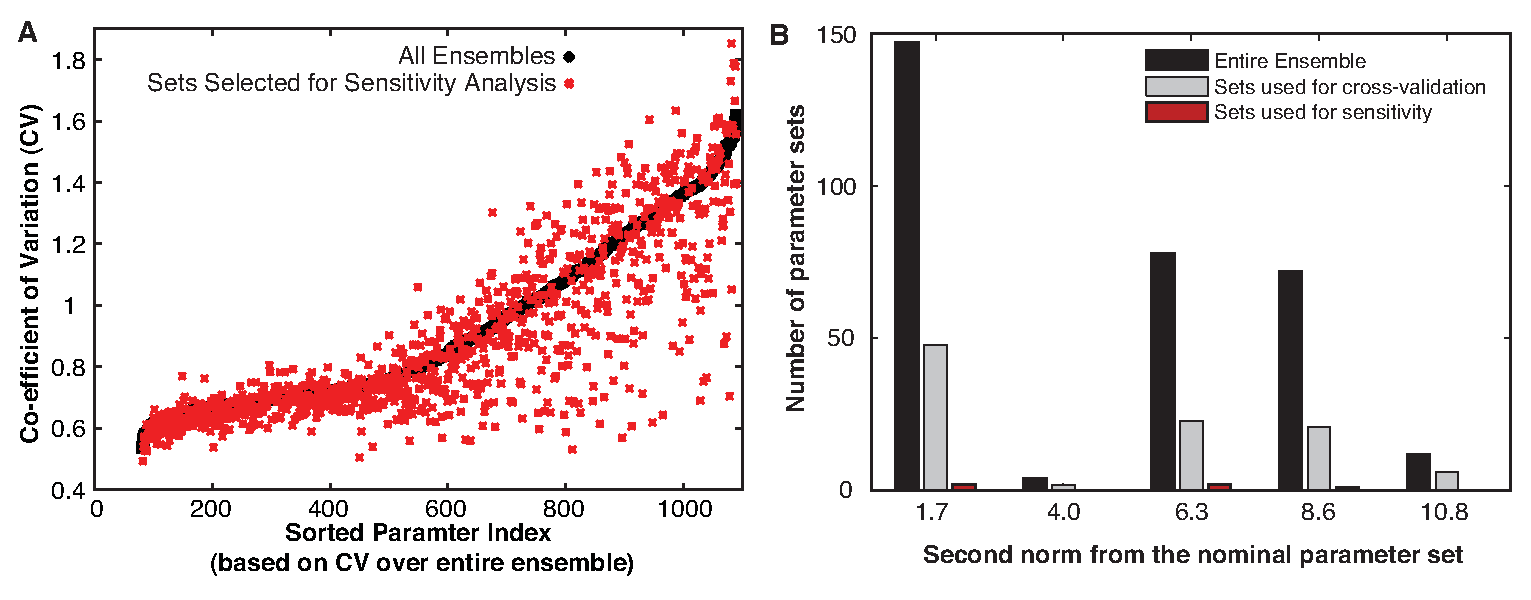
\epsfig{file=./Supp_Figures/Para_S1.eps,width=1.0\textwidth}
	\caption{ POETs generated an ensemble of models that predicted approximately 94\% of the objective functions with a significantly higher likelihood than a random control. (A) The coefficient of variation (CV) for the model parameters ranged from 0.5 - 1.6, where approximately 65\% of the parameters were constrained with a CV $\leq$ 1.0 (black dots). (B) We selected five parameter sets (red dots in A) for further analysis based on CV and distance from the nominal parameter set (based on second norm).}
	\label{fg:Para_S1}
\end{figure}

\begin{figure}\centering
	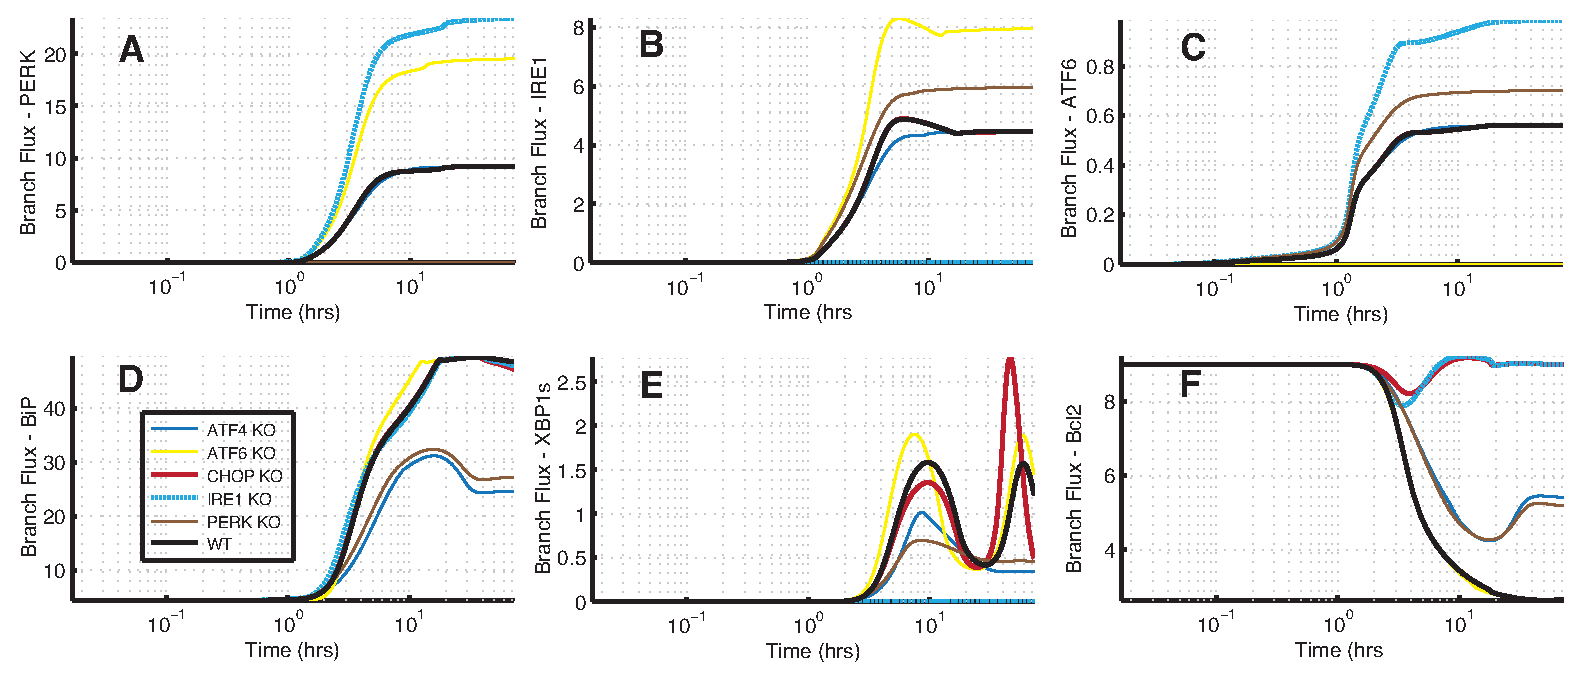
\epsfig{file=./Supp_Figures/Flux_S1.eps,width=1.0\textwidth}
	\caption{Signal flow analysis using simulated knockout (KO) of key proteins on the UPR system: Simulation results suggest that the three branches in UPR fire simultaneously with varying rates and the state of the cell in terms of adaptation, alarm or apoptosis is a result of counteracting effects of these three prongs of UPR signaling. 
	(A-C) The counteracting effects is seen when knockout of one ER stress transducer leads to enhancement of the other branches of UPR. 
	(D) ATF4, cleaved ATF6 and XBP1s act as integrators of the signals coming from all the three branches of UPR and furthermore leads to regulation of BiP, thereby leading to a negative feedback or control of UPR signal. PERK and ATF4 KO studies revealed a slower and lower amount of BiP production ($\sim$ 50\%) as compared to WT. However, ATF6 or IRE1 KO did not affect BiP regulation as compared to WT. 
	(E) Regulation of BiP was the critical regulator of spliced XBP1 (XBP1s), which in turn acts as a key marker of progression through different stages of UPR. 
	(F) PERK and ATF4 KO lead to delay in the onset of apoptosis (marked by slower and lower reduction of Bcl2 levels. This effect could be attributed to the lack of CHOP mediated branch of Bcl2 regulation. On the other hand, IRE1 and CHOP KO leads to drastic reduction in apoptosis (marked by little or no change of Bcl2 levels). CHOP KO, implicated the importance of CHOP in the down-regulation of Bcl2. IRE1 KO implicated the critical role of IRE1-TRAF2 mediated route of apoptosis. 
Overall flux analysis highlighted the extensive amount of crosstalk within the three branches of the UPR network.}
\label{fg:Flux_Supp_Fig1}
\end{figure}

\begin{figure}\centering
	\epsfig{file=./Supp_Figures/Sens_S1.eps,width=1.0\textwidth}
	\caption{Plot of species sensitivity at earlier (0-2 hrs) versus later (6-8 hrs) time points: Sensitivity analysis was conducted over discrete two hour time windows thereby revealing the time evolution of the importance of UPR network modules. We found that signal integration via the transcriptional activity of ATF6, ATF4 and XBP1s along with RCAN1 and cIAP role in apoptosis were significantly more important at 6-8 hrs as compared to 0-2 hrs time window. This is consistent with the dominant role of the negative feedback via the transcriptional regulation of BiP in UPR. Interestingly, the majority of species rankings were similar as seen in the cluster in the grey box.}
	\label{fg:Sens_S1}
\end{figure}

\begin{figure}\centering
	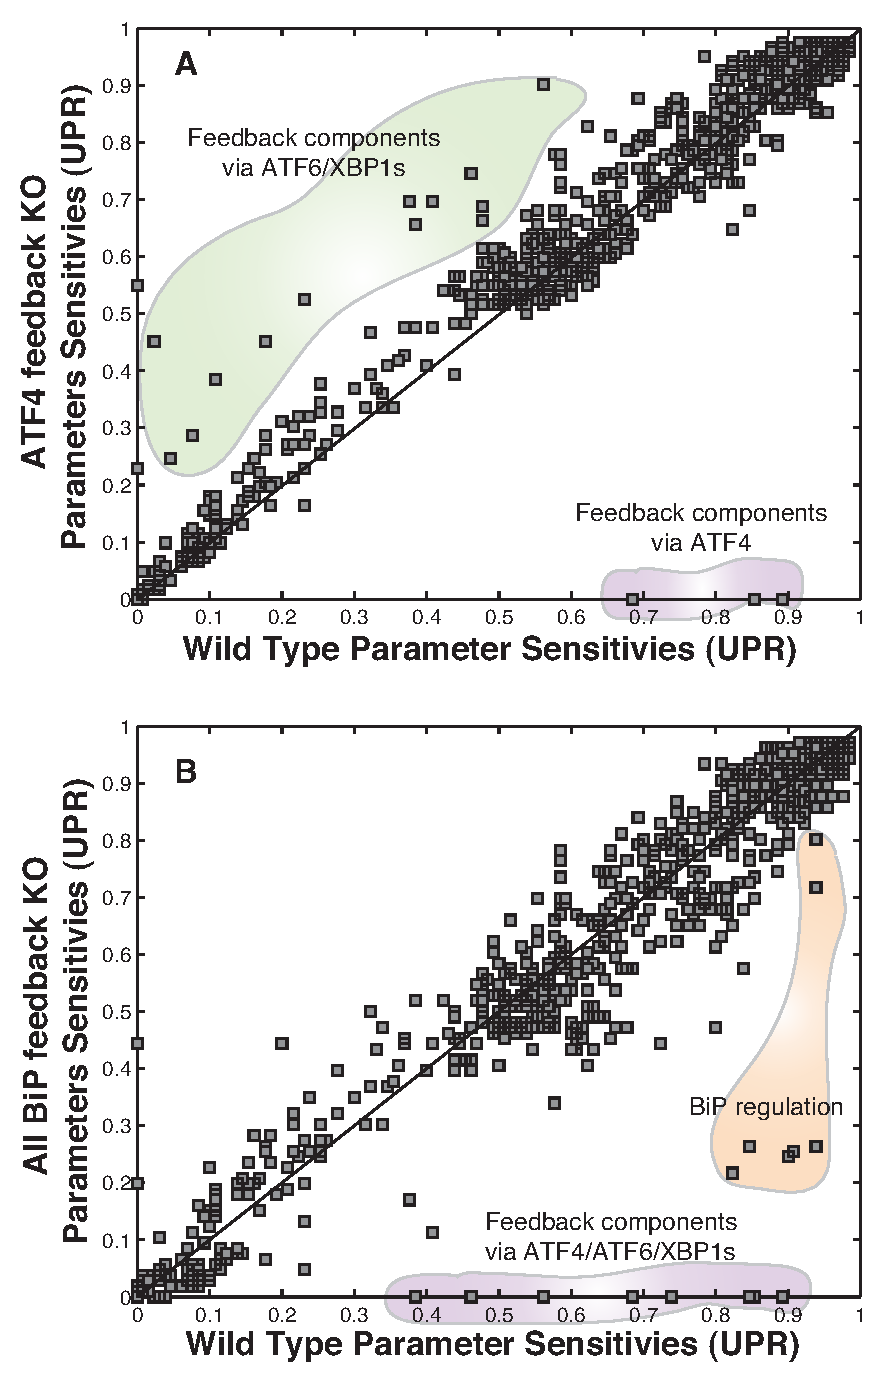
\epsfig{file=./Supp_Figures/Sens_S3.eps,width=0.6\textwidth}
	\caption{Plot of parameter sensitivity with APAF-1 feedback KO and all BiP feedback KO: Upon knockout of any individual feedback branch like that of ATF4, ATF6 and XBP1s, the system overall remains equally robust. However the sensitivity of the alternate feedback components increases. This was most evident upon ATF4 feedback KO. 
	(A) We saw increase in sensitivity of feedback components associated with XBP1s and ATF6. Upon ATF6 and XBP1s feedback KO, there wasn't much change in terms of sensitivity of the system (data not shown). This further attests the key regulatory effect of ATF4 in mediating the positive BiP feedback which is an essential component of the adaptation phase of UPR. 
	(B) When we completely knockout all the feedback branches of BiP in the adaptation phase, the system overall becomes relatively more robust. We distinctly saw a major shift of sensitivity of BiP upon removal of positive feedback. Overall $\sim$ 54 \% of the parameters were differentially less sensitive upon removal of BiP feedback as compared to WT. This brings to light how the presence of BiP feedback makes the system more susceptible/sensitive to perturbations.}
	\label{fg:Sens_S3}
\end{figure}


\begin{figure}\centering
	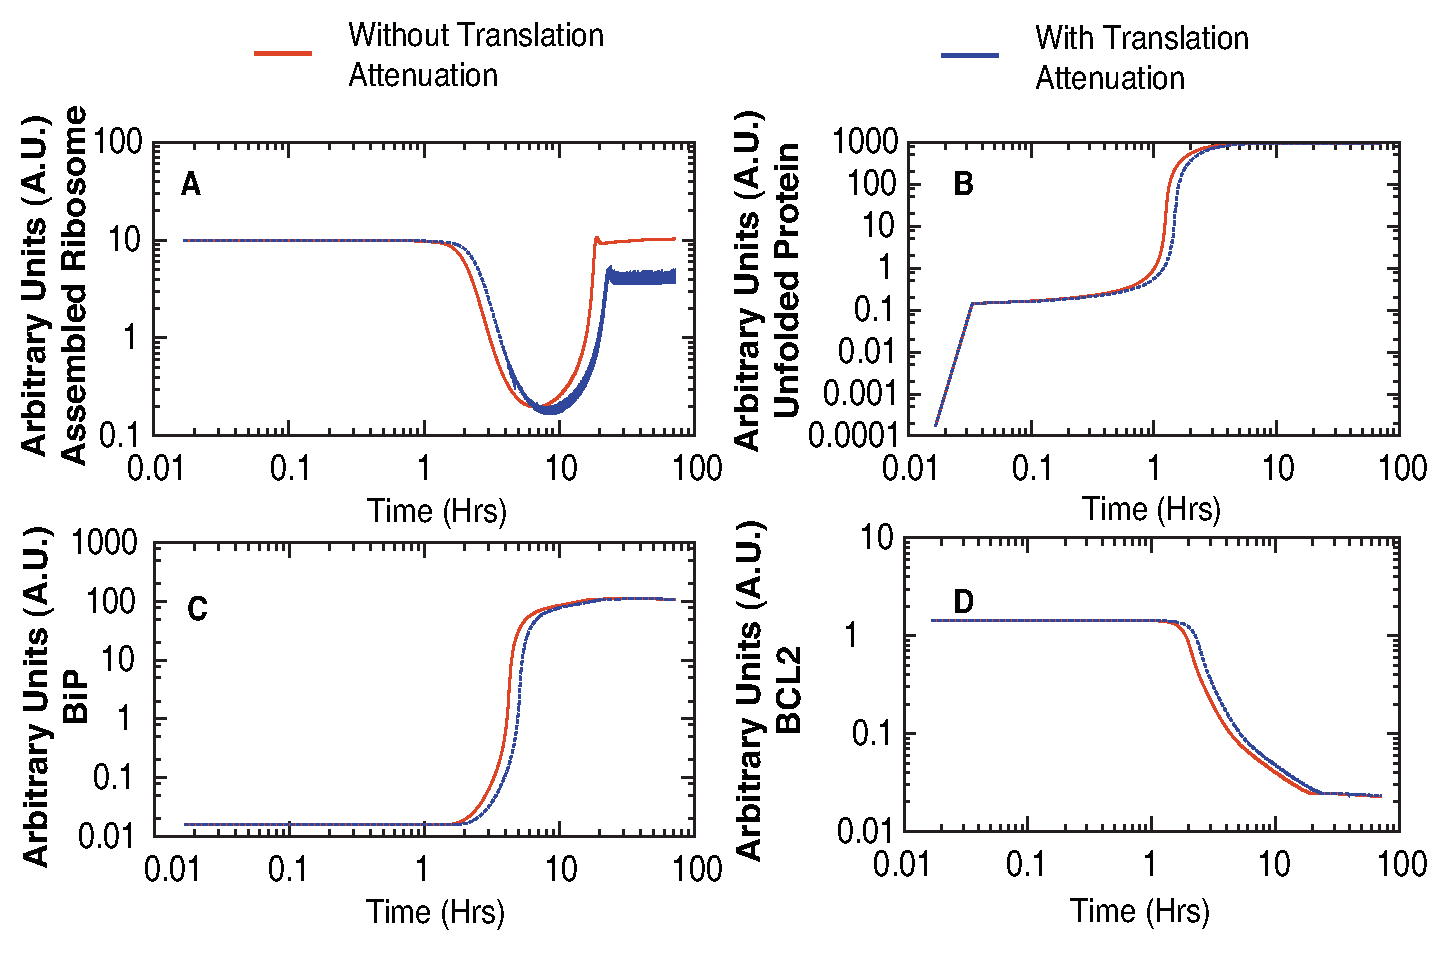
\epsfig{file=./Supp_Figures/TRANS_S1.eps,width=1.0\textwidth}
	\caption{Simulations with translation attenuation built in the model: One of the key aspects which was not included in the current model was translation attenuation. So we simulated that to identify that there isnt much of a change overall in the system except for the tad bit delay in the onset of the responses. }
	\label{fg:Trans_S1}
\end{figure}

\begin{figure}\centering
	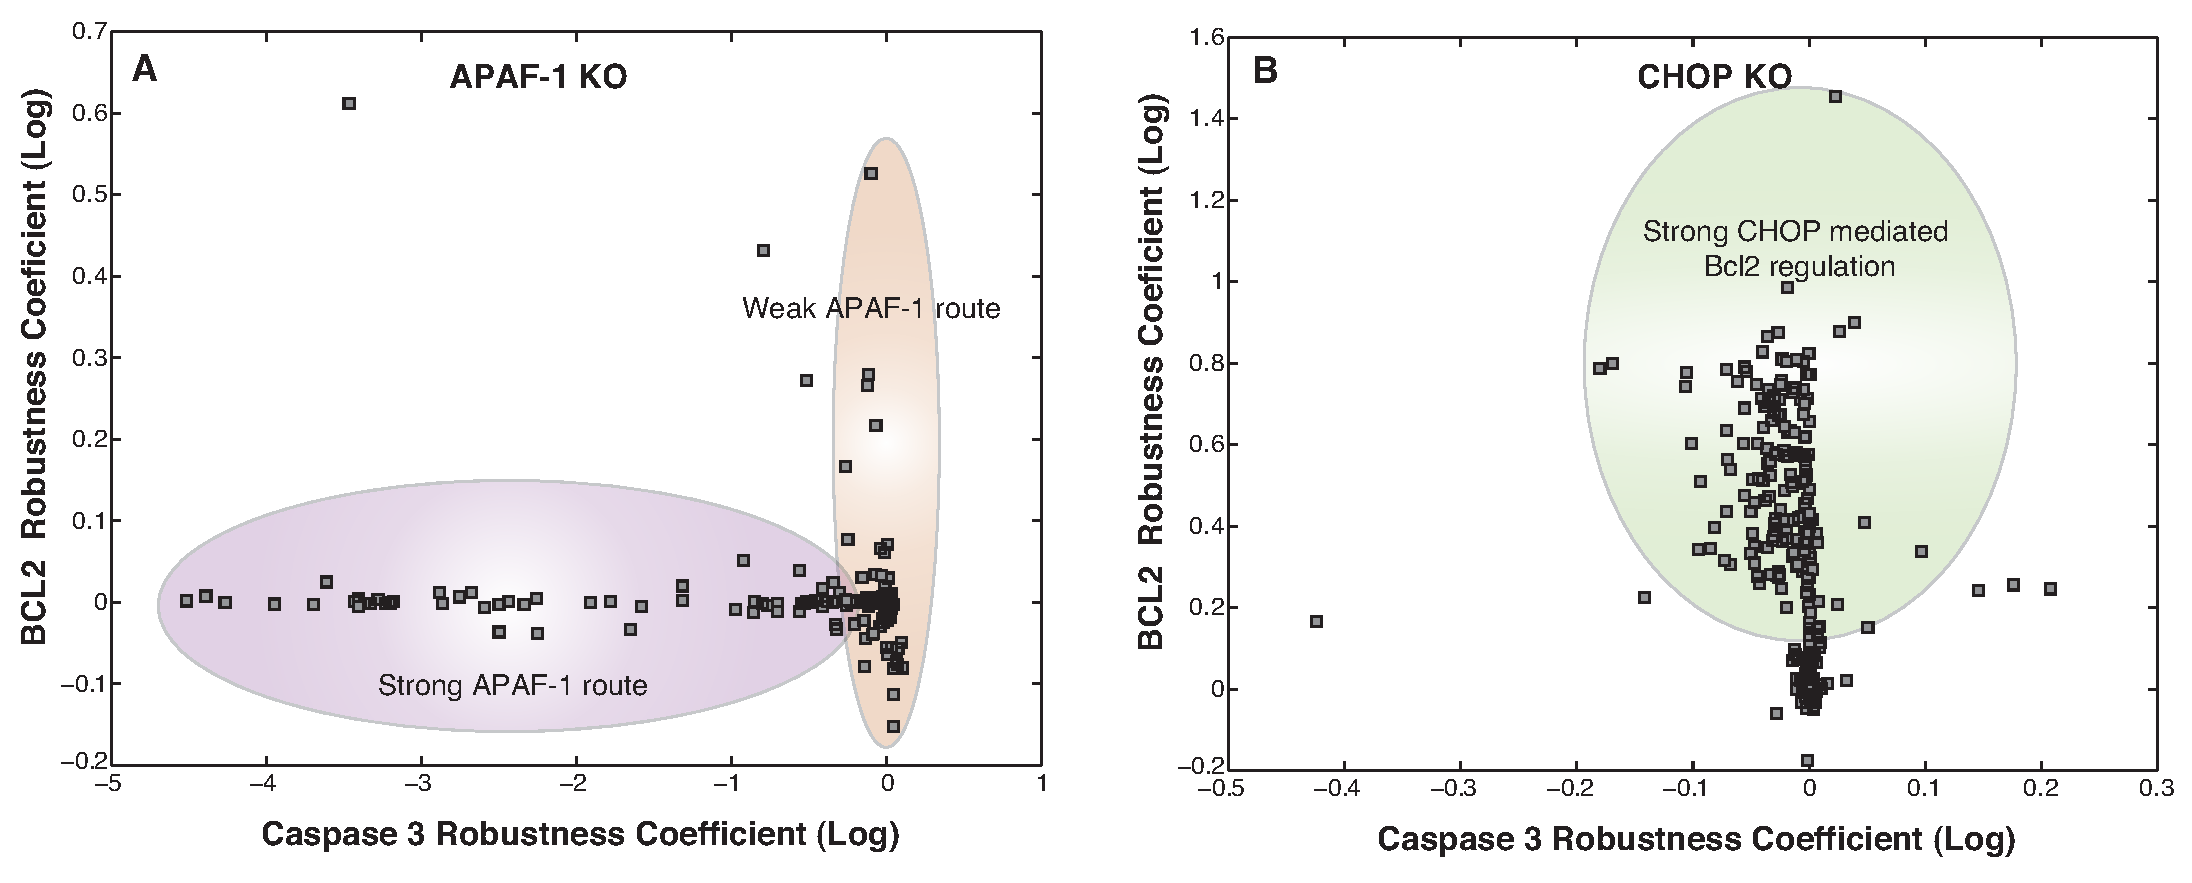
\epsfig{file=./Supp_Figures/COUP_S1.eps,width=1.0\textwidth}
	\caption{Survival-death phenotypic plane for APAF-1 and CHOP KOs over the entire ensemble: (A) With APAF-1 KO, we found that there were two populations of cells in the ensemble: population 1 where APAF-1 was the dominant regulator of cell-death (marked by enhanced reduction in caspase 3 upon APAF-1 KO) and population 2 where APAF-1 is not the most dominant regulator (marked by reduced effect on Caspase 3 upon APAF-1 KO). (B) Upon CHOP KO, we identified two distinct populations within the ensembles. One with a strong effect of CHOP mediated down-regulation of Bcl2 (marked by $\sim$ 10 fold increase in Bcl2 levels) and the other with very little effect of CHOP on Bcl2 levels. This behavior could be attributed to other conflicting means of regulation of Bcl2 levels.}
	\label{fg:COUP_S1}
\end{figure}

\begin{figure}\centering
	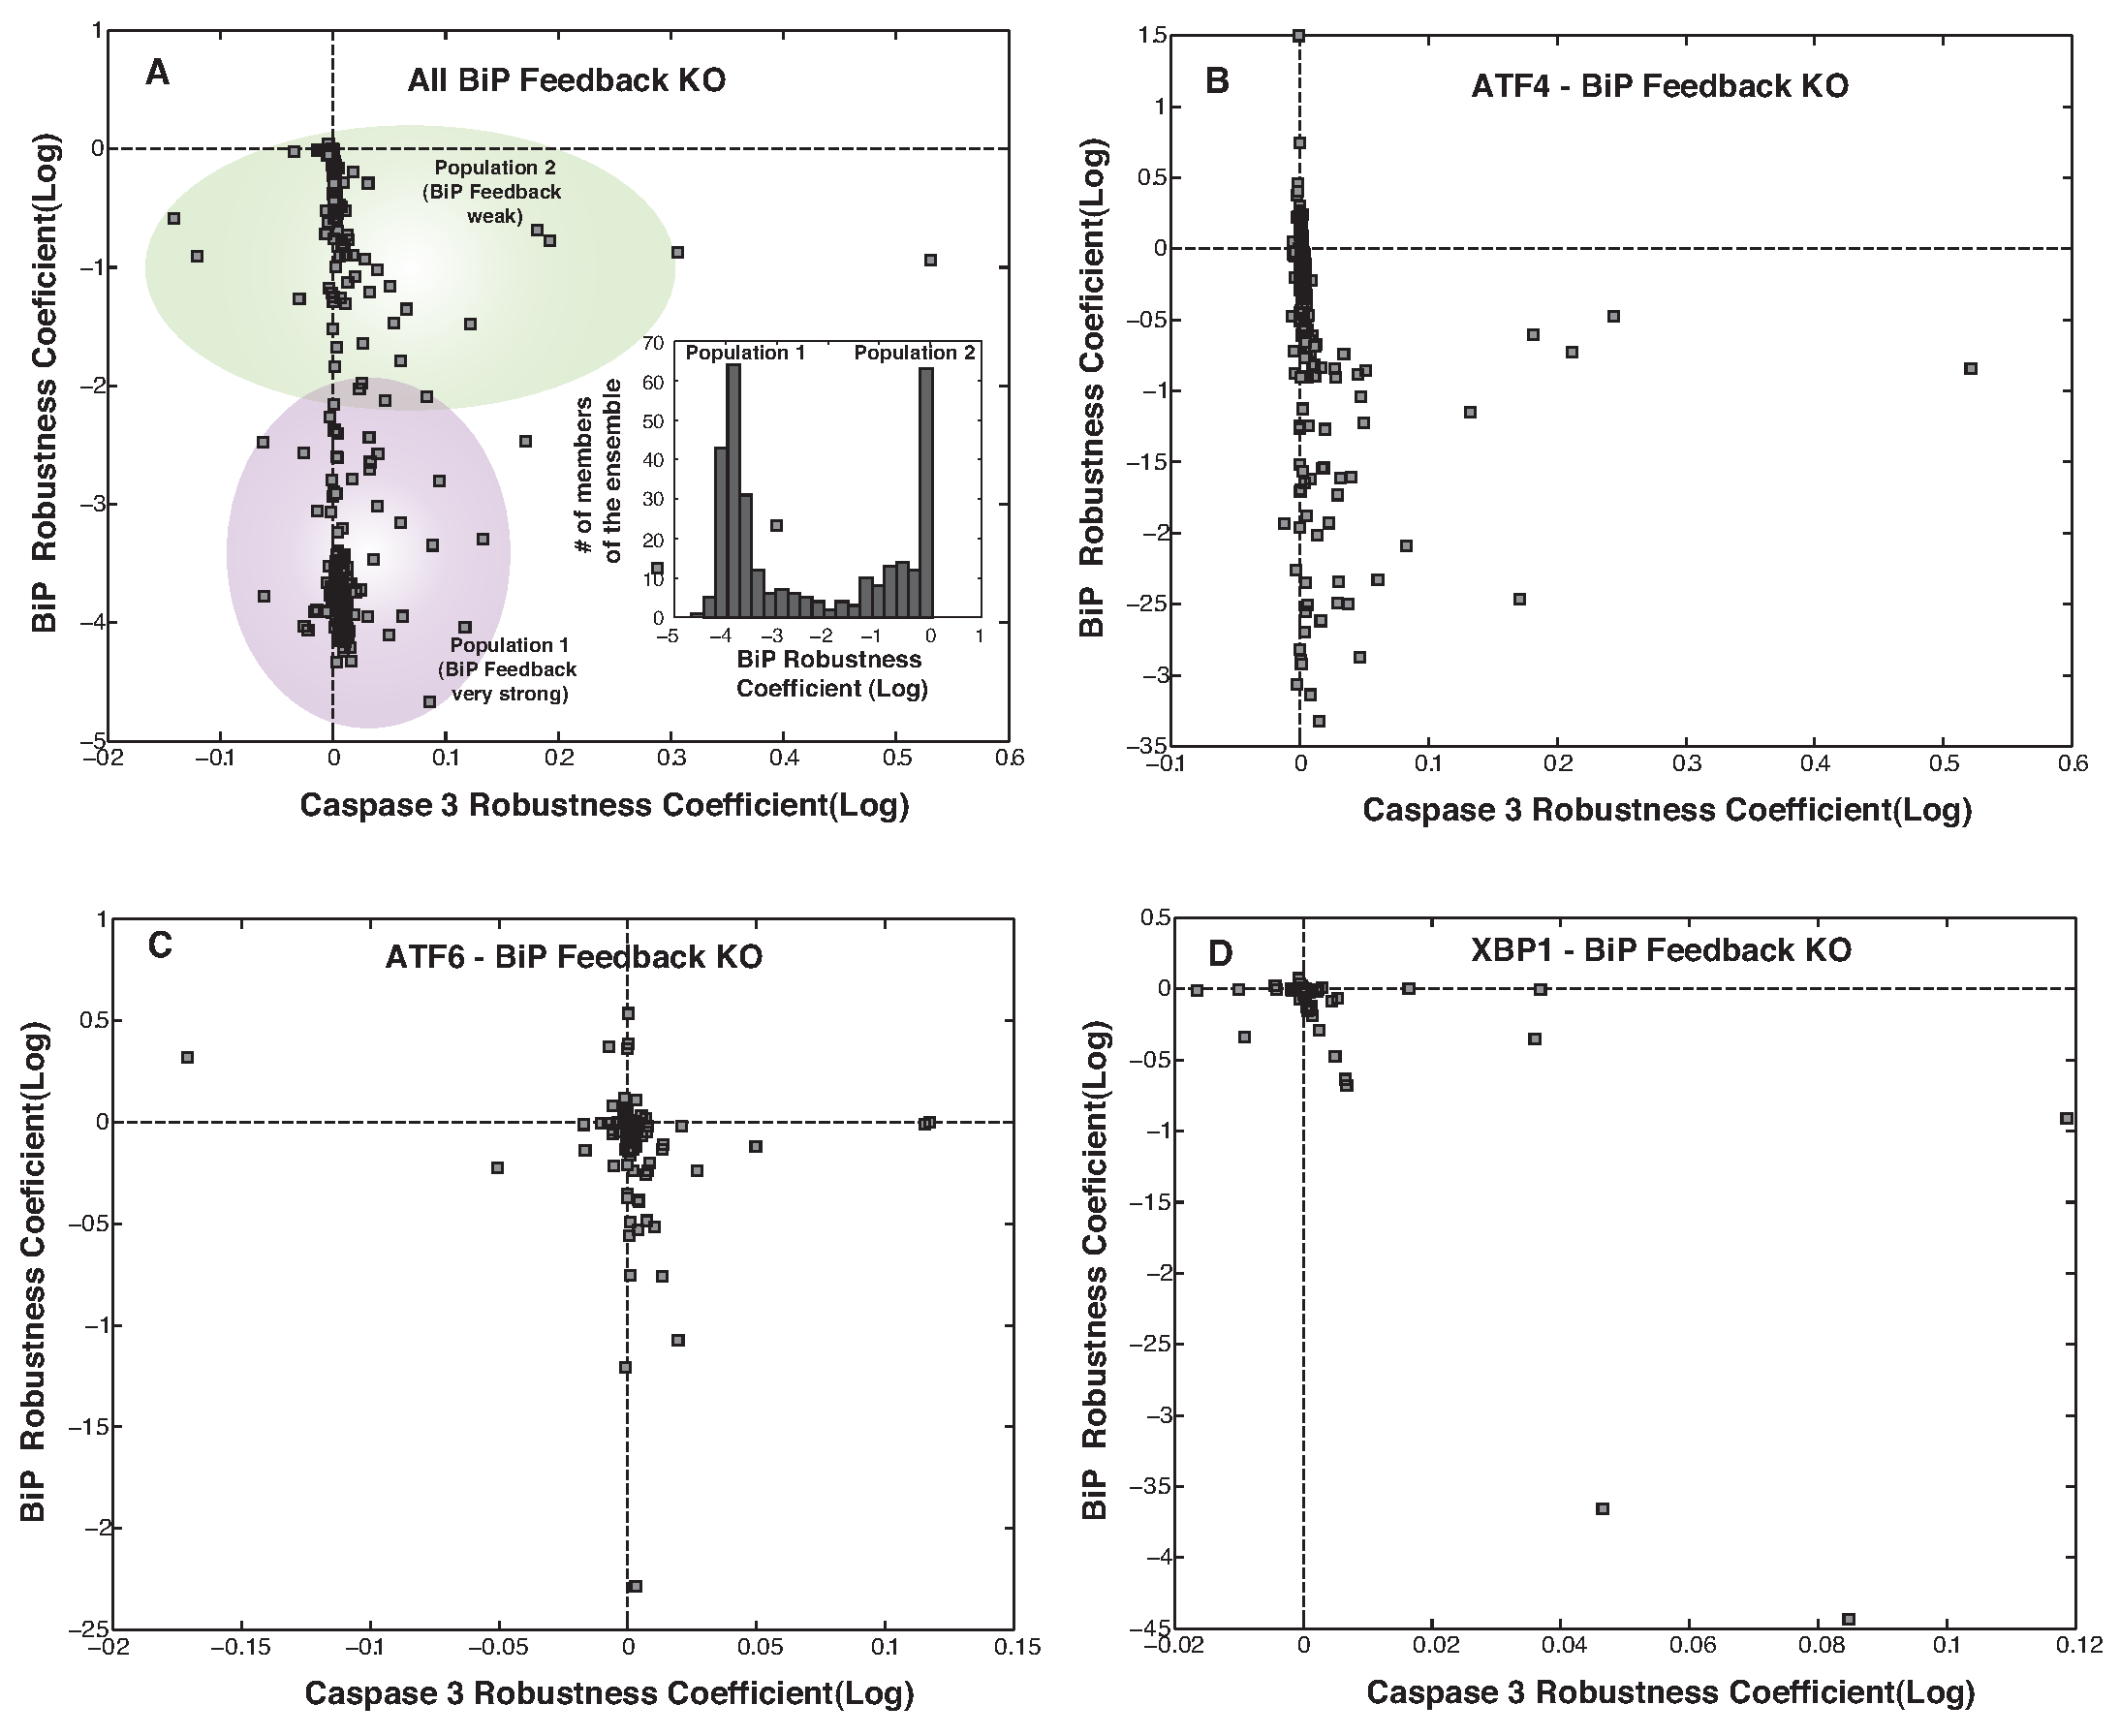
\epsfig{file=./Supp_Figures/COUP_S2.eps,width=1.0\textwidth}
	\caption{To further investigate the implications of the feedback regulation of BiP via ATF4/ATF6/XBP1s, we simulated KOs of these components over the entire ensemble. (A) Upon KO of all branches of BiP feedback, we found overall reductions of BiP levels. However, there were two distinct sub-populations. One with a $\sim$ 10 fold reduction in BiP levels while the other had $\sim$ 1000 fold reduction in BiP levels. These two populations could resemble two distinct operational paradigms within UPR. In the first mode of operation feedback regulation of BiP is really strong so when we knockout BiP feedback we have drastic reductions in BiP levels and ultimately a stronger and faster UPR response. (B) ATF4 mediated feedback KO led to significant amount of reduction in BiP levels thereby highlighting the significance of ATF4 in BiP feedback. (C-D) However, KO of ATF6 and XBP1s mediated feedback of BiP was seen to have little effect (as marked by robustness coefficients for BiP).}
	\label{fg:COUP_S2}
\end{figure}